\documentclass[12pt]{article}
\usepackage{fullpage,graphicx,amsmath,amsfonts,forest,listings,xcolor}
\usepackage[hidelinks]{hyperref}
\usepackage[small,bf]{caption}

\definecolor{bgcolor}{rgb}{0.95,0.95,0.95}
\lstdefinestyle{mystyle}{
basicstyle=\footnotesize\ttfamily,
backgroundcolor=\color{bgcolor},
keywordstyle=\color{violet},
stringstyle=\color{red},
commentstyle=\color{gray},
showstringspaces=false,
numbers=left,
frame=line
}
\lstset{
style=mystyle,
breaklines=true,
postbreak=\mbox{\textcolor{red}{$\hookrightarrow$}\space}
}

\bibliographystyle{acm}

\title{
Attribute-Based Encryption
}
\author{
Yao-Wen Chang, Ju-Ting Chen, Shao-Hsuan Chu \\
Instructor: Chun-I Fan \\
\\
National Sun Yat-sen University
}

\begin{document}
\maketitle
\begin{abstract}
In this work, we will briefly discuss the evolution of attribute-based encryption (ABE) and why we need ABE. We will further discuss the different schemes of ABE including key-policy and ciphertext-policy ABE. In the experiment, we’ll design an on-line chatting room service program and grant it the ability to use ABE to transmit messages between multiple users. We’ll see how well ABE suits for such multicast service using a well-designed policy and reduces the overhead on the sending host by distributing the same copy of ciphertexts to multiple receivers.
\end{abstract}
\newpage
\tableofcontents
\newpage


\section{Introduction}
It is a trend nowadays that everyone uses the Internet very often. However,  there is a significant risk of personal privacy leak in the Internet since everyone can sniff the packets on the Internet channel. This has given rise to various encryption methods in which plaintexts are encrypted before leaving the sending host, and the decryption is performed at the receiving host. Each encryption method serves a different purpose depending on the requirements and environments. For example, symmetric encryption is used when there’s a way to securely exchange keys in advance. Asymmetric encryption, a.k.a. public-key encryption is used when the public key infrastructure (PKI) is available in an organization. One of the variants of asymmetric encryption, attribute-based encryption (ABE), has been envisioned as a promising cryptographic primitive for realizing secure and flexible access control. ABE has significant advantage over the traditional PKI primitives as it achieves flexible one-to-many encryption instead of one-to-one. In which, the attributes of the sender and receiver are used for encryption instead of using public-private key pairs. The concept is a generalization of the predecessor of ABE, identity-based encryption (IBE). While in IBE, a user attribute is used to generate the key for encryption and decryption, in ABE, multiple attributes can be used to generate the key. Therefore ABE is also called fuzzy identity-based encryption.

Two main components of ABE, attribute and policy, determine how the plaintexts are encrypted and who gets the ability to decrypt the message. A policy typically uses a tree structure containing the logic relations between attributes. ABE can be classified based on who defines the policy. Two dominant schemes are key-policy ABE (KP-ABE) and ciphertext-policy ABE (CP-ABE). We’ll review these models in the next section.

\section{Related works}
\subsection{Asymmetric encryption}
Asymmetric encryption solves the problem of key sharing by using different keys for encryption and decryption. A central authority is also required to distribute the public-private key pairs. At the sending side, the sender would have to decide who is the receiver and acquire the public key of which from the central authority, then use this key to encrypt the messages to be sent. The ciphertext generated in the last step would travel through a possibly non-secure channel and finally arrive at the receiving host. At the receiving side, upon receiving the ciphertext, the receiver uses its own private key to decrypt and obtain the plaintext messages. Aside from the need of a public key infrastructure (PKI), one major limitation in this model is that the ciphertext depends on the public key of the receiver, that is to say, if the sender wants to distribute the messages to multiple receivers, it needs to perform $N$ encryption based on $N$ public keys of $N$ users, respectively. This yields a big overhead on the sending side. Moreover, the receiver cannot decrypt the message without its private key, but there’s no guarantee that the receiver would never lose its private key. Think about an example in real life. When we want to send a mail to our friend, we would like to send it to the person rather than the person who has the key to the mailbox. With the concerns above, identity-based encryption was proposed.
\subsection{Identity-based encryption}
To deal with the overhead of PKI and burden on senders, IBE, Shamir \cite{Sha:85}, is a solution for only grappling with the overhead of PKI. How it operates will be discussed in the Figure \ref{fig:IBE}. IBE systems allow anyone to generate a public key from a known identity value, like the email of the identity. First, Bob will register to the private key generator (PKG) and show its identity. Then, PKG will generate the master public key and master private key. PKG only keeps the master private key, and publishes the master public key. Every party can compute the public key based on the master public key and identity value. Then, Alice can encrypt the message and send the encrypted message. If the receiver wants to decrypt the message, it can fetch the private key by showing its identification.

IBE has some issues with security. Firstly, if PKG cannot provide a secure channel delivering the private key, then everyone who can forge the identification of the receiver can get the private key. Second, PKG generates private keys for users, and it can also decrypt or sign the message without authorization. Hence, IBE cannot support non-repudiation. It seems like IBE is a perfect cryptography, nevertheless, the sender should also need to compute each time when sending the same message to different receivers. Therefore, attribute-based encryption will be adopted by the user.

\begin{figure}
\begin{center}
    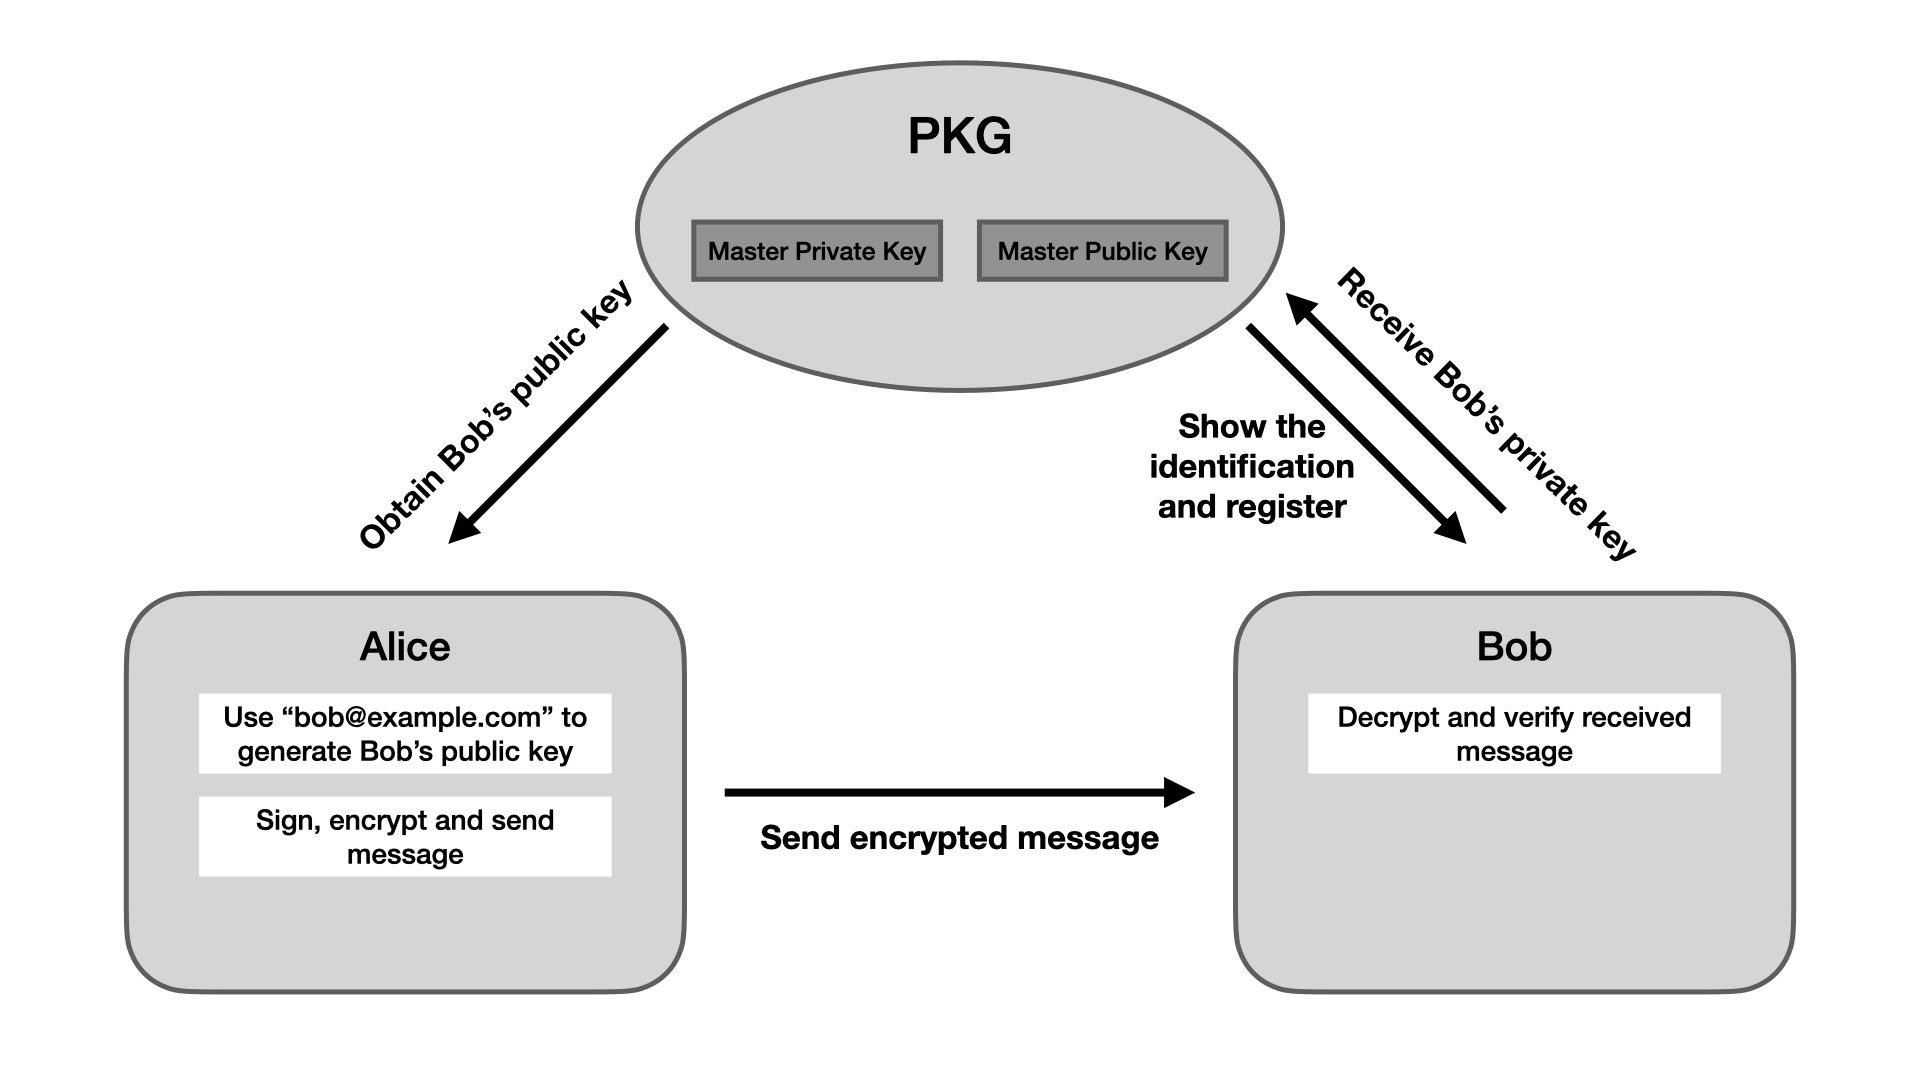
\includegraphics[width=1.0\textwidth]{assets/figures/IBE}
\end{center}
\caption{Operation of identity-based encryption}
\label{fig:IBE}
\end{figure}


\section{Attribute-based encryption}
Attribute-based encryption(ABE) was first proposed by Sahai and Waters in 2005 \cite{SW:05}, and the earliest prototype of ABE is inherited from IBE. However ABE solves the problem of the inability to have a one-to-many user model from IBE. ABE access rules defined by the user when encrypting data are not based on the identity of the recipient. It takes attributes as the public key and associates the ciphertext and user’s secret key with attributes, so that it can support expressive access control policies.  One can encrypt a message to any user satisfying the boolean formula. For instance, a party might want to share animal information with only users that have the attribute of  “Biologist” and the attribute “researcher”.  However it might have some problems when the same organizations join the same projects. Because one needs a single authority that is able to verify attributes across different organizations and issue private keys to every user in the system, unlike traditional public systems. It is because of this feature that ABE allows fine-grained access control of data, which is more flexible than traditional public encryption systems and reduces the complexity of user management. It also reduces the complexity of user management. ABE can be divided into key-policy ABE (KP-ABE) and ciphertext-policy ABE (CP-ABE), These are the two main categories of ABE. The difference between the two is whether the access rules are embedded in a key or a cipher.

\subsection{Key-policy attribute-based encryption}
Key-Policy Attribute-Based Encryption(KP-ABE) was first proposed by Goyql \cite{GPSW:06}, in which an access rule is linked to the private key and the ciphertext is linked to a set of attributes. That is to say, the receiver can define the access rule composed of attribute set and policy and the sender encrypts messages with an attribute set. For example, suppose there is an animal information A is encrypted with the attributes {“2000”, “mammals” , “body temperature”} and another animal information B is encrypted with the attributes {“2000”, “reptiles”, "body temperature”}. If the access rule of Alice is “2000” AND “ mammals”, Alice is able to access  information A but not reptiles in 2000. And if the access rule of Bob is “2000” AND “ body temperature”, then Bob can access both data A and B.
\subsection{Ciphertext-policy attribute-based encryption}
Ciphertext-Policy Attribute-Based Encryption (CP-ABE) was proposed by Bethencourt \cite{BSW:07} and in contrast to KP-ABE, CP-ABE links the ciphertext to an access rule and the private key to a set of attributes, which means sender can decide who is able to access the informations, making a big difference between KP-ABE and CP-ABE . For instance, when an animal information is encrypted, and the access rule is  “School A” AND ( “researcher” OR “biologist”), which means that any researcher or biologist in School A can access the animal information according to the attributes they hold. While those researchers or biologists at School B or School C cannot access the information due to non-compliance with the access rules. Not to mention those whose access rule is not even researcher or biologist.
\subsection{Searchable attribute-based encryption}
While CP-ABE seems to be more realistic for practical uses since the sender can define the entire access structure, attribute set and policy, and that the very scheme we’ll use in our experiment of on-line chatting service. However, the KP-ABE is more suitable for searchable encryption in comparison to CP-ABE \cite{HQZH:14}. We’ll elaborate on the reason in the next paragraph.

Searchable encryption is an encryption algorithm with an additional searchable property. The common application is cloud storage service, in which the data owner stores their encrypted data on a third-party cloud storage. With ABE, the data owner can encrypt the data with some keywords as attributes, and the keywords can be used to search for this data later on. Once the encrypted data is stored in the cloud, various users, including the owner, can construct the access rules composed of logic relations between selected keywords to search for the data. In KP-ABE, the receivers do have the ability to construct their own access rule. This enables the downloaders to build a complicated and precise search policy. 

To wrap up, when a user wants to search for and download data encrypted with some keywords from the cloud storage, the user constructs the access rule of keywords and sees if it can decrypt the data. Note that in the practical implementation, instead of downloading all the data and examining on the downloader’s host, the private key generated by the access rule should be uploaded to the cloud and check if it can decrypt the data, i.e., performing search, on the cloud. Of course, besides the keywords, the data owner can encrypt the data with other attributes such as valid username or IP address that have permission to this data. If the access rule provided by the downloader cannot meet the decryption requirements, then it is as-if not found in the traditional search scheme.

\section{Experiments}
In the following experiments, we'll use the OpenABE library, zeutro \cite{Zeu:18}, as our back-end encryption/decryption engine. We'll first look at two minimal examples enforcing KP-ABE and CP-ABE, respectively. Then we would discuss the design and usage of a secure on-line chatting service. We'll use C++ to develop the programs, and the following header and namespaces are used in every examples.
\begin{lstlisting}[language=c++]
#include <openabe/openabe.h>
using namespace oabe;
using namespace oabe::crypto;
\end{lstlisting}
\subsection{Implementing KP-ABE}
As we've seen, In KP-ABE, the sender encrypted the messages with a set of attributes, and the receiver generates the private key with a self-define access rule composed of attribute set and policy. In other words, the ciphertext is linked to a set of attributes while the private key is linked to an access rule. We'll first initialize and distribute the master public key by
\begin{lstlisting}[language=c++]
InitializeOpenABE();
cout << "Initializing KP-ABE" << endl;
OpenABECryptoContext kpabe("KP-ABE");
kpabe.generateParams();
string mpk, msk;
kpabe.exportPublicParams(mpk);
kpabe.exportSecretParams(msk);
cout << "Master public key:\n" << mpk << endl;
cout << "Master secret key:\n" << msk << endl;
\end{lstlisting}
After established a secure channel between users and the PKG, the sender can now encrypt the messages with some attributes, we provides two set of attributes for later comparison.
\begin{lstlisting}[language=c++]
string pt = "hello world!";
vector<string> attributes = {"|attr1|attr2|", "|attr3|attr4|"};
vector<string> ct(attributes.size());
for (size_t i = 0; i < attributes.size(); i++) {
    kpabe.encrypt(attributes[i], pt, ct[i]);
    cout << "Attribute set" << i+1 << ":\n\"" << attributes[i] << "\"\n";
    cout << "Plaintext:\n" << pt << endl;
    cout << "Ciphertext:\n" << ct[i] << "\n\n";
}
\end{lstlisting}
At the same time, the receiver may send its access rule to the PKG and get back a private key for the later decryption. We assume there's only receiver and would like to see whether the access rule match to the attribute sets above.
\begin{lstlisting}[language=C++]
kpabe.enableKeyManager("user");
string policy = "(attr1 and attr3) or attr2", sk;
kpabe.keygen(policy, "key0");
kpabe.exportUserKey("key0", sk);
// *** transmission ***
kpabe.importUserKey("key0", sk); // import to the receiving host
cout << "Receiver's policy:\n\"" << policy << "\"\n";
cout << "Generated key:\n" << sk << endl;
\end{lstlisting}
Finally, the receiver can decrypt the incoming messages with the generated private key. Note that we need to catch the exception where the decryption failed.
\begin{lstlisting}[language=C++]
string rePt;
bool result;
for (size_t i = 0; i < ct.size(); i++) {
    cout << "Sender's attributes "<<i+1<<":\n\""<< attributes[i]<<"\"\n";
    cout << "Decrypt:\n";
    try {
        result = kpabe.decrypt(ct[i], rePt);
        if (result && pt == rePt) cout << "Recovered message: " << rePt << "\n\n";
    } catch (oabe::ZCryptoBoxException& ex) {
        cout << ex.what() << endl;
        cout << "Failed to recover the message.\n\n";
    }
}
\end{lstlisting}
\subsubsection{Results}
\begin{lstlisting}[language=sh]
Testing KP-ABE

################## Setup ##################
Master public key:
AAAAFqpv (truncated)
Master secret key:
AAAAFqpv (truncated)
###########################################


################# Encrypt #################
Attribute set1:
"|attr1|attr2|"
Plaintext:
hello world!
Ciphertext:
AAABKaET (truncated)
Attribute set2:
"|attr3|attr4|"
Plaintext:
"hello world!"
Ciphertext:
AAABKaET (truncated)
#########################################


################# KeyGen ##################
Receiver policy:
"(attr1 and attr3) or attr2"
Generated key:
AAAAF6pv (truncated)
#########################################


################# Decrypt #################
Sender attributes 1:
"|attr1|attr2|"
Decrypt:
Found Key: 'key0' => '(attr1 and attr3) or attr2'
Recovered message: "hello world!"

Sender attributes 2:
"|attr3|attr4|"
Decrypt:
Key Manager could not find an appropriate key to decrypt!
Failed to recover the message.

#########################################
\end{lstlisting}
The source code for this and the next sub-sections is available in our GitHub repository\footnote{Minimal KP-ABE and CP-ABE examples \url{https://github.com/ernestchu/abe-examples}.}.
\subsection{Implementing CP-ABE}
While sharing most of the code with KP-ABE example, in CP-ABE example, the sender encrypts the messages with an access rule, and the receiver define a set of attributes.
\begin{lstlisting}[language=c++]
cout << "\n################# Encrypt #################\n";
string pt = "hello world!";
vector<string> policies = {"attr1 or attr2", "attr1 and attr2"};

cout << "\n################# KeyGen ##################\n";
cpabe.enableKeyManager("user");
string recvAttrs = "|attr1|", sk;
cpabe.keygen(recvAttrs, "key0");
\end{lstlisting}
\subsubsection{Results}
\begin{lstlisting}[language=sh]
Testing CP-ABE

################## Setup ##################
Master public key:
AAAAFqpv (truncated)
Master secret key:
AAAAFqpv (truncated)
###########################################


################# Encrypt #################
Policy 1:
"attr1 or attr2"
Plaintext:
"hello world!"
Ciphertext:
AAABq6ET (truncated)

Policy 2:
"attr1 and attr2"
Plaintext:
"hello world!"
Ciphertext:
AAABrKET (truncated)

#########################################


################# KeyGen ##################
Receiver attributes:
"|attr1|"
Generated key:
AAAAF6pv (truncated)
#########################################


################# Decrypt #################
Policy 1: (the receiver should not know this)
"attr1 or attr2"
Decrypt:
Found Key: 'key0' => '|attr1|'
Recovered message: "hello world!"

Policy 2: (the receiver should not know this)
"attr1 and attr2"
Decrypt:
Key Manager could not find an appropriate key to decrypt!
Failed to recover the message.

#########################################
\end{lstlisting}

\subsection{A secure on-line chatting service}
In this experiment, we designed a secure on-line chatting service that consists of a message server and one or more clients that can talk to each other. No message would leave a client's host unencrypted. A message would stay encrypted even if it is cached on the server. For the simplicity, only the receiver's username is used as attributes for the encryption on the sending side. Being a message-exchanging server, it is also play the role of the PKG as well. In such architecture, the server does have the ability to decrypt all the messages. However, it is complete viable to separate the message server and the PKG, but we're not going to do that in this work for the sake of simplicity.

A client may send a message to one or more users as long as he/she knows their username. This is also known as a multi-casting service. This is also the reason why ABE is suitable for the encryption task in this service. For example, suppose a user want to send a message to some users, including, “James“, “Durant“, “Harden“ and “Curry“. On the sending side, the sender defines an access rule: USERNAME = “James“ OR “Durant“ OR “Harden“ OR “Curry“, and encrypts the message he wants to send with such access rule. Any client whose username matches to one of them would be able to decrypt the message. Most importantly, the server only have to compute one copy of the ciphertext, greatly reducing the overhead on the sending host.

\begin{lstlisting}[language=c++]
// perform ABE encryption
for (const auto& receiver : receivers)
    policy += (" or " + receiver);

// make only one copy of ciphertext
abe.encrypt(policy, message, ciphertext);
for (const auto& receiver : receivers)
    this->network.send( // only send back the first msg
        receiver,
        ciphertext,
        (int)(receiver!=receivers[0])
    );
\end{lstlisting}

The source code is available in our GitHub repository\footnote{Secure on-line chatting service \url{https://github.com/ernestchu/on-line-chatting-service/tree/abe}.}. A demonstration video describing the usage is also available on YouTube\footnote{Demonstration video for secure on-line chatting service \url{https://youtu.be/S-j5kQz_-7Y}.}. See Figure \ref{fig:client} for the client sample output, and Figure \ref{fig:server} for the server's sample output.

\begin{figure}
\begin{center}
    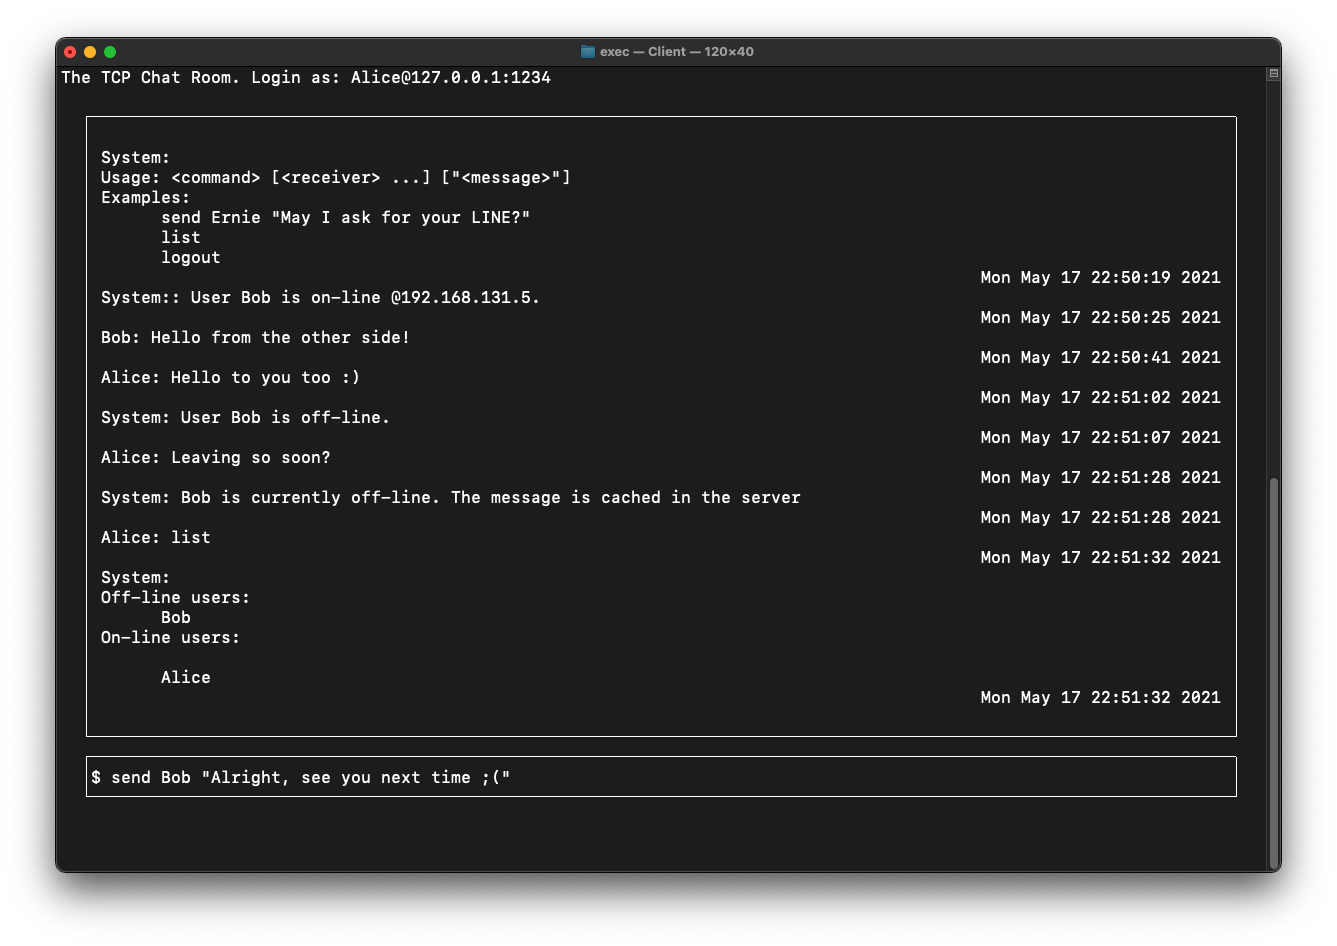
\includegraphics[width=1.0\textwidth]{assets/figures/client}
\end{center}
\caption{The client in the secure on-line chatting service}
\label{fig:client}
\end{figure}

\begin{figure}
\begin{center}
    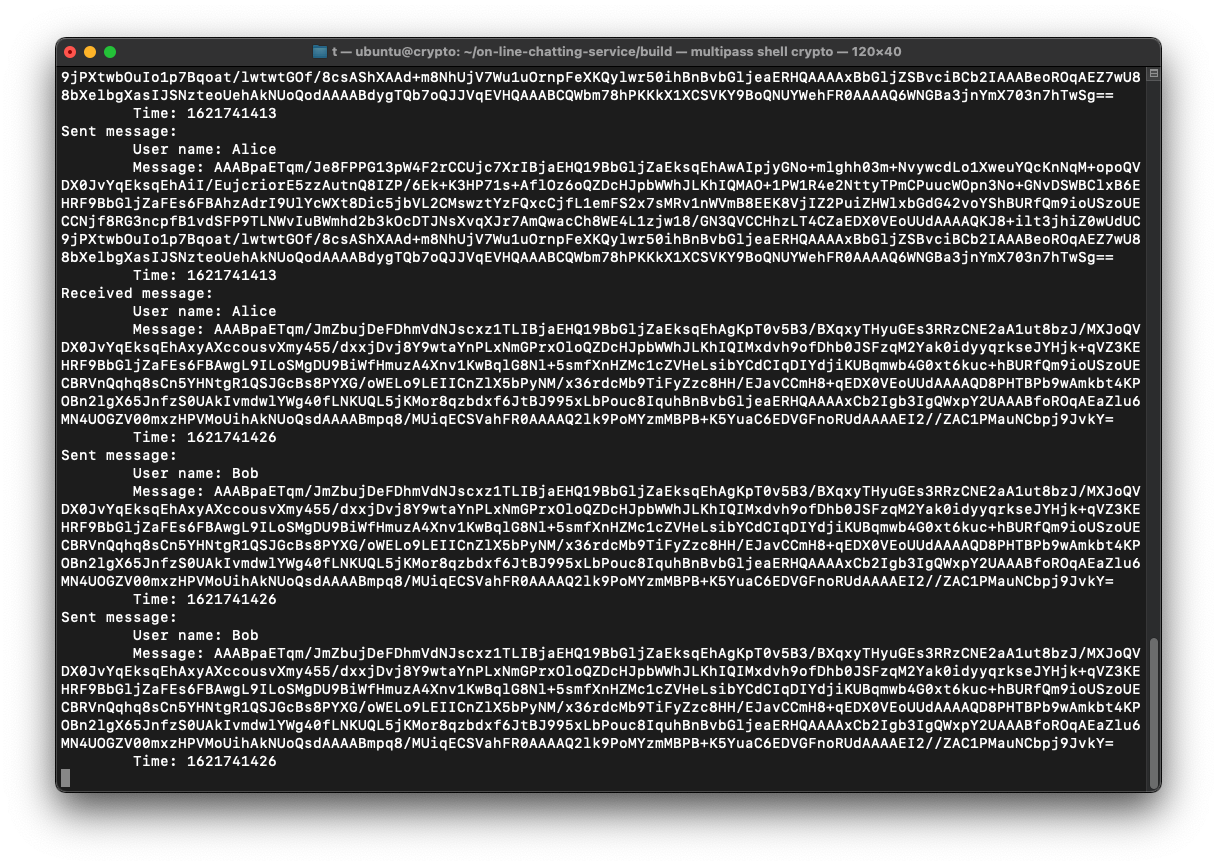
\includegraphics[width=1.0\textwidth]{assets/figures/server}
\end{center}
\caption{The server in the secure on-line chatting service}
\label{fig:server}
\end{figure}

\newpage
\bibliography{References}

\end{document}
